% !TeX root = mos-he.tex

%%%%%%%%%%%%%%%%%%%%%%%%%%%%%%%%%%%%%%%%%%%%%%%%%%%%%%%%%%%%%%%%

\begin{prob}{לדגום עם או בלי החזרות?}{D,S}{(Should you sample with or without replacement?)}

בכד 
$A$
נמצאים
$2$
כדורים אדומים ו-%
$1$
כדור ירוק, ובכד 
$B$
נמצאים
$101$
כדורים אדומים ו-%
$100$
כדורים ירוקים. בחר כד אחד בצורה אקראי ושלוף שני כדורים באופן אקראי מהכד שנבחר. אתה מנצח אם אתה מזהה נכון אם כדורים נשלפו מכד 
$A$
או כד
$B$.

חשב את ההסתברויות לניצחון של כל אחד מהחוקים שלהן וקבע איזה חוק נותן את ההסתברות הגבוהה ביותר לניצחון.

\que{1}
אתה מחזיר את הכדור הראשון לפני השליפה השנייה.

\que{2} 
אתה לא מחזיר את הכדור הראשון לפני השליפה השנייה.

\que{3}
לאחר נשלף הכדור הראשון אתה יכול להחליט אם להחזיר אותו או לא.

\textbf{רמז:} 
כאשר מחשבים הסתברויות:
\[
\disfrac{101}{201}\approx \disfrac{100}{201} \approx \disfrac{100}{200} \approx \disfrac{1}{2}\,.
\]
\end{prob}

\vspace{-7ex}

\solution{}

יש ארבע תוצאות שנסמן
$RR, RG, GR, GG$.
לכל אחד מהחוקים נחשב את ההסתברויות המתנות של ארבעת התוצאות תלוי בזהות הכד 
$A$
או
$B$
שנבחר תחילה. אחר כך נכפיל את ההסתברויות ב-%
$1/2$
כדי לקחת בחשבון את הבחירה האקראית של הכד.

\ans{1}
שליפה עם החזרה:
\[
\renewcommand*{\arraystretch}{1.5}
\begin{array}{lcccc}
P(RR|A) &=& \frac{2}{3} \cdot \frac{2}{3} &=& \frac{4}{9}\\
P(RR|B) &=& \frac{1}{2} \cdot \frac{1}{2} &=& \frac{1}{4}\\
\hline
P(RG|A) &=& \frac{2}{3} \cdot \frac{1}{3} &=& \frac{2}{9}\\
P(RG|B) &=& \frac{1}{2} \cdot \frac{1}{2} &=& \frac{1}{4}\\
\hline
P(GR|A) &=& \frac{1}{3} \cdot \frac{2}{3} &=& \frac{2}{9}\\
P(GR|B) &=& \frac{1}{2} \cdot \frac{1}{2} &=& \frac{1}{4}\\
\hline
P(GG|A) &=& \frac{1}{3} \cdot \frac{1}{3} &=& \frac{1}{9}\\
P(GG|B) &=& \frac{1}{2} \cdot \frac{1}{2} &=& \frac{1}{4}\end{array}
\]
אם התוצאה היא
$RR$
ההסתברות שכד 
$A$
נבחר
($4/9$)
גבוהה מהסתברות שכד
$B$
נבחר
($1/4$);
אחרת, ההסתברות ש-%
$B$
נבחר גבוהה יותר. לכן:
\[
P(\textrm{ניצחון})=\frac{1}{2}\left(\frac{4}{9} + \frac{1}{4}+ \frac{1}{4}+ \frac{1}{4}\right)=\disfrac{43}{72}\approx 0.5972\,.
\]

\ans{2}
שליפה ללא החזרה:
\[
\renewcommand*{\arraystretch}{1.5}
\begin{array}{lcccc}
P(RR|A) &=& \frac{2}{3} \cdot \frac{1}{2} &=& \frac{1}{3}\\
P(RR|B) &=& \frac{1}{2} \cdot \frac{1}{2} &=& \frac{1}{4}\\
\hline
P(RG|A) &=& \frac{2}{3} \cdot \frac{1}{2} &=& \frac{1}{3}\\
P(RG|B) &=& \frac{1}{2} \cdot \frac{1}{2} &=& \frac{1}{4}\\
\hline
P(GR|A) &=& \frac{1}{3} \cdot 1 &=& \frac{1}{3}\\
P(GR|B) &=& \frac{1}{2} \cdot \frac{1}{2} &=& \frac{1}{4}\\
\hline
P(GG|A) &=& \frac{1}{3} \cdot 0 &=& 0\\
P(GG|B) &=& \frac{1}{2} \cdot \frac{1}{2} &=& \frac{1}{4}
\end{array}
\]
אם התוצאה היא
$GG$
ההסתברות שכד
$B$
נבחר גבוהה יותר (כמובן!) מההסתברות שכד
$A$
נבחר; אחרת, ההסתברות שכד 
$A$
נבחר גבוהה יותר. לכן:
\[
P(\textrm{win})=\frac{1}{2}\left(\frac{1}{3} + \frac{1}{3}+ \frac{1}{3}+ \frac{1}{4}\right)=\frac{5}{8}=0.6250\,,
\]
שהיא גבוהה יותר מההסתברות לניצחון כאשר שליפה היא עם החזרה.

\ans{3} 
ההחלטה נעשית על סמך התוצאות מהשליפה הראשונה.

אם השליפה הראשונה היא מכד
$A$
ההסתברויות חייבות להיות מותנות בהחלטה להחזיר או לא. שליפה הראשונה היא מכד
$B$
לא משפיעה על ההסתברויות בגלל הקירוב ברמז.
\[
\renewcommand*{\arraystretch}{1.5}
\begin{array}{lcccc}
P(RR|A,w) &=& \frac{2}{3} \cdot \frac{2}{3} &=& \frac{4}{9}\\
P(RR|A,w/o) &=& \frac{2}{3} \cdot \frac{1}{2} &=& \frac{1}{3}\\
P(RR|B) &=& \frac{1}{2} \cdot \frac{1}{2} &=& \frac{1}{4}\\
\hline
P(RG|A,w) &=& \frac{2}{3} \cdot \frac{1}{3} &=& \frac{2}{9}\\
P(RG|A,w/o) &=& \frac{2}{3} \cdot \frac{1}{2} &=& \frac{1}{3}\\
P(RG|B) &=& \frac{1}{2} \cdot \frac{1}{2} &=& \frac{1}{4}\\
\hline
%\end{array}
%\]
%\[
%\renewcommand*{\arraystretch}{1.5}
%\begin{array}{lcccc}
P(GR|A,w) &=& \frac{1}{3} \cdot \frac{2}{3} &=& \frac{2}{9}\\
P(GR|A,w/o) &=& \frac{1}{3} \cdot 1 &=& \frac{1}{3}\\
P(GR|B) &=& \frac{1}{2} \cdot \frac{1}{2} &=& \frac{1}{4}\\
\hline
P(GG|A,w) &=& \frac{1}{3} \cdot \frac{1}{3} &=& \frac{1}{9}\\
P(GG|A,w/o) &=& \frac{1}{3} \cdot 0 &=&0\\
P(GG|B) &=& \frac{1}{2} \cdot \frac{1}{2} &=& \frac{1}{4}\\\end{array}
\]
אם כדור אדום נשלף ראשונה אזי 
$\frac{4}{9}>\frac{1}{4}$
ו-%
$\frac{2}{9}<\frac{1}{4}$
עם החזרה, לעומת
$\frac{1}{3}>\frac{1}{4}$
ו-%
$\frac{1}{3}>\frac{1}{4}$
ללא החזרה, לכן הכדור השני יכול לעזור בזיהוי הכד רק אם השליפה נעשית 
\textbf{עם}
החזרה: אם אדום כד
$A$
ואם ירוק כד
$B$.
נבחר שליפה עם החזרה ו:
\[
P(\textrm{ראשון אדום אם ניצחון})=\frac{1}{2}\left(\frac{4}{9}+\frac{1}{4}\right)=\frac{25}{72}\,.
\]
אם כדור ירוק נשלף ראשון אזי
$\frac{2}{9}<\frac{1}{4}$
ו-%
$\frac{1}{9}<\frac{1}{4}$
עם החזרה, לעומת
$\frac{1}{3}>\frac{1}{4}$
ו-%
$0<\frac{1}{4}$
ללא החזרה, לכן הכדור השני יכול לעזור בזיהוי הכד רק אם השליפה נעשית 
\textbf{בלי}
החזרה ו:
\[
P(\textrm{ראשון ירוק אם ניצחון})=\frac{1}{2}\left(\frac{1}{3}+\frac{1}{4}\right)=\frac{7}{24}\,.
\]
ההסתברות לניצחון היא:
\[
P(\textrm{ניצחון})=\frac{25}{72} + \frac{7}{24}=\frac{23}{36}\approx 0.6389\,.
\]
ההסתברות הגבוהה ביותר לניצחון מתקבלת כאשר ההחלטה לשלוף עם או בלי החזרה מתקבל בהתאם לתוצאה של השליפה הראשונה.

\textbf{סימולציה}
\selectlanguage{english}
\begin{verbatim}
With replacement:
Expectation of winning = 0.5972
Average wins           = 0.5976
Without replacement:
Expectation of winning = 0.6250
Average wins           = 0.6207
Decide after first draw:
Expectation of winning = 0.6389
Average wins           = 0.6379
\end{verbatim}
\selectlanguage{hebrew}

%%%%%%%%%%%%%%%%%%%%%%%%%%%%%%%%%%%%%%%%%%%%%%%%%%%%%%%%%%%%%


\begin{prob}{הקלפי}{S}{(The ballot box)}

שתי מועמדות 
$A$
ו-%
$B$
מתמודדות בבחירות. 
$A$
קיבלה
$a$
קולות ו-%
$B$
קיבלה
$b$
קולות,
$a>b$.
הקולות נספרים אחד-אחד וסכומי הביניים
$(a_i,b_i), 1\leq i \leq a+b$
מתעדכנים לאחר ספירת כל קול. מה ההסתברות שעבור לפחות
$i$
אחד,
$a_i=b_i$?

\que{1} 
פתור עבור
$a=3, b=2$
על ידי הכנת רשימה
$(a_i,b_i)$
עבור
$1\leq i\leq 5$.

\que{2} 
פתור עבור כל
$a>b$.

\textbf{רמז 1:} 
מה ניתן להגיד על זהות המועמדת שמובילה עד לתיקו 
\textbf{ראשון}?

\textbf{Hint 2:}
מה החשיבות של הקול הראשון שנספר.
\end{prob}

\solution{}

\ans{1}
מספר הדרכים לסדר את סכומי הביניים הוא
${5\choose 2}={5\choose 3}=10$ 
כי המיקום הקולות עבור מועמדת אחת קובע את מיקום הקולות של המועמדת השנייה. בטבלה שלהלן רשומים הסידורים האפשריים של הקולות וסכומי הביניים כאשר התיקו הראשון מודגש:
\begin{center}
\begin{minipage}{.48\textwidth}
\[
\begin{array}{ccccc}
A & A & A & B & B\\
A & A & B & A & B\\
A & B & A & A & B\\
B & A & A & A & B\\%\hline
A & A & B & B & A\\
A & B & A & B & A\\
B & A & A & B & A\\%\hline
A & B & B & A & A\\
B & A & B & A & A\\%\hline
B & B & A & A & A
\end{array}
\]
\end{minipage}
\hspace{-4em}
\begin{minipage}{.48\textwidth}
\[
\begin{array}{rrrrr}
%(4,5)&
(1,0) & (2,0) & (3,0) & (3,1) & (3,2)\\
%(3,5)&
(1,0) & (2,0) & (2,1) & (3,1) & (3,2)\\
%(2,5)&
(1,0) & \mathbf{(1,1)} & (2,1) & (3,1) & (3,2)\\
%(1,5)&
(0,1) & \mathbf{(1,1)} & (2,1) & (3,1) & (3,2)\\%\hline
%(3,4)&
(1,0) & (2,0) & (2,1) & \mathbf{(2,2)} & (3,2)\\
%(2,4)&
(1,0) & \mathbf{(1,1)} & (2,1) & (2,2) & (3,2)\\
%(1,4)&
(0,1) & \mathbf{(1,1)} & (2,1) & (2,2) & (3,2)\\%\hline
%(2,3)&
(1,0) & \mathbf{(1,1)} & (1,2) & (2,2) & (3,2)\\
%(1,3)&
(0,1) & \mathbf{(1,1)} & (1,2) & (2,2) & (3,2)\\%\hline
%(1,2)&
(0,1) & (0,2) & (1,2) &  \mathbf{(2,2)} & (3,2)
\end{array}
\]
\end{minipage}
\end{center}
קיימים מצבי תיקו בכל הסידורים פרט לשני הראשונים ולכן:
\[
P(\textrm{קולות}\;(3,2)\;\textrm{עם תיקו קיים})=\disfrac{8}{10}=\disfrac{4}{5}\,.
\]

\ans{2} 
נתחיל את הפתרון עם דיון איך לגשת לפתרון של השאלה השנייה. הנה מספר סידורים עבור 
$(a,b)=(3,2)$
עד לקבלת
\textbf{התיקו הראשון}:
\[
\begin{array}{rrrrr|rrrrr}
\multicolumn{5}{c|}{A \;\textrm{leads until tie}} &
\multicolumn{5}{c}{B \;\textrm{leads until tie}}\\\hline
A & B &&& &B & A & & &\\
A & A & B & B && B & B & A & A&\\
\end{array}
\]
לכל סידור בו 
$A$
מובילה עד לתיקו הראשון, קיים סידור שהוא תמונת ראי בו 
$B$
מובילה עד לקבלת התיקו הראשון. השיקוף מתקבל על ידי החלפת כל 
$A$
ב-%
$B$
ולהפך.

לפני התיקו הראשון אחת מהמועמדות חייבת להוביל. אם הקול הראשון שנספר הוא עבור 
$B$
חייב להיות תיקו בהמשך הספירה כי
$a>b$.

ההסתברות שהקול הראשון היא עבור 
$B$
היא:
\[
P(B\;\textrm{עבור ראשון קול})=\frac{b}{a+b}\,.
\]
על ידי שיקוף המיקומים של הקולות, מספר הסידורים שמובילים לתיקו שמתחילים בקול עבור
$A$
שווה למספר הסידורים שמובילים לתיקו שמתחילים בקול עבור
$B$. 
לכן:
\[
P(\textrm{תיקו קיים })=2\cdot\frac{b}{a+b}\,.
\]
בדיקה:
\[
P(\textrm{קולות}\;(3,2)\;\textrm{עם תיקו קיים})=2\cdot\frac{2}{2+3}=\frac{4}{5}\,.
\]

\textbf{סימולציה}
\selectlanguage{english}
\begin{verbatim}
For a =  3, b =  2:
Probability of a tie = 0.8000
Proportion of ties   = 0.8118
For a = 10, b =  8:
Probability of a tie = 0.8889
Proportion of ties   = 0.8977
For a = 20, b = 18:
Probability of a tie = 0.9474
Proportion of ties   = 0.9354
\end{verbatim}
\selectlanguage{hebrew}


%%%%%%%%%%%%%%%%%%%%%%%%%%%%%%%%%%%%%%%%%%%%%%%%%%%%%%%%%%%%%

\begin{prob}{תיקו בהשוואת מטבעות}{D,S}{(Ties in matching pennies)}

הטל זוג מטבעות הוגנות
$N$
פעמים עבור
$N$
זוג, ורשום את מספר הפעמים שהזוגיות היא זוגי (עץ-עץ או פלי-פלי) ומספר ההפעמים שהזוגיות היא אי-זוגי (עץ-פלי או פלי-עץ). מה ההסתברות לקבל תיקו (לא כולל התיקו 
$0-0$
בהתחלה)?

\que{1}
פתור עבור 
$N=4$
על ידי רישום כל התוצאות האפשריות.

\que{2} 
פתור עבור
$N=6$
על ידי פיתוח נוסחה להסתברות.

\que{3} 
פתח נוסחה עבור כל
$N$
זוגי.

\que{4}
הסבר מדוע ההסתברות למספר אי-זוגי
$N+1$
שווה להסתברות של המספר הזוגי
$N$.

\textbf{רמז:}
השתמש בפתרון לבעיה~22.
\end{prob}

\solution{}

\ans{1} 
נסמן את ההטלות עם זוגיות זוגי ב-%
$E$
וההטלות עם זוגיות אי-זוגי ב-%
$O$.
בעשרה מתוך שש עשרה סידורי ההטלות יש תיקו (מודגש):
\begin{center}
\begin{tabular}{llllllll}
EEEE & EEEO & EEOE & \textbf{EEOO} & \textbf{EOEE} & \textbf{EOEO} &\textbf{EOOE} & \textbf{EOOO}\\
\textbf{OEEE} & \textbf{OEEO} & \textbf{OEOE} & \textbf{OEOO} & \textbf{OOEE} & OOEO&OOOE & OOOO
\end{tabular}
\end{center}

\ans{2}
לפי בעיה~22:
\begin{equation}\label{eq.coins-ties}
P(i\;\textrm{בהטלה תיקו})=
\left\{
\begin{array}{ll}
2i/N &\textrm{if}\; i\leq N/2\\
2(N-i)/N& \textrm{if}\; i\geq N/2\,,
\end{array}
\right.
\end{equation}
כי בבעיית הקלפי הראנו שהערך הנמוך יותר קובע את ההסתברות.

החישובים שלהלן די מסובכים לכן נצדיק כל חישוב לפרטים.

ההסתברות ל-%
$i$
זוגיים ניתן על ידי ההתפלגות הבינומית:
\begin{equation}\label{eq.coins00}
P(i\;\textrm{זוגיים})=\dischoose{N}{i} \left(\disfrac{1}{2}\right)^i \left(\disfrac{1}{2}\right)^{N-i}=\dischoose{N}{i} \left(\disfrac{1}{2}\right)^N =  2^{-N}\dischoose{N}{i}\,.
\end{equation}
ההסתברות לתיקו היא הסכום מעל 
$i$
של ההסתברות לקבל 
$i$
זוגיים כפול ההסתברות לתיקו בהטלה ה-%
$i$
(משוואה%
~\ref{eq.coins-ties}). For $N=6$:
\begin{equation}\label{eq.coins0}
P(\textrm{ties})=2\cdot 2^{-6}\left[
\frac{0}{6}\dischoose{6}{0} + \frac{1}{6}\dischoose{6}{1} +
\frac{2}{6}\dischoose{6}{2} + \frac{3}{6}\dischoose{6}{3} +
\frac{2}{6}\dischoose{6}{4} + \frac{1}{6}\dischoose{6}{5} +
\frac{0}{6}\dischoose{6}{6}
\right]\,.
\end{equation}
משוואה%
~\ref{eq.coins1}
נובעת ממשוואה%
~\ref{eq.coins0}
על ידי השמטת שני הגורמים שהם אפס, כתיבת ה
\L{combination???}
עם עצרת, צימצום 
$1/6$
מ-%
$6!$:
\begin{equation}\label{eq.coins1}
P(\textrm{ties})=2^{-5}\left[
1\cdot\disfrac{5!}{1!5!} + 2\cdot\disfrac{5!}{2!4!} +
3\cdot\disfrac{5!}{3!3!} + 2\cdot\disfrac{5!}{4!2!} +
1\cdot\disfrac{5!}{5!1!}
\right]\,.
\end{equation}
משוואה%
~\ref{eq.coins2}
מתקבלת מצימצום
$i$
מ-%
$i!$:
\begin{equation}\label{eq.coins2}
P(\textrm{ties})=2^{-5}\left[
\disfrac{5!}{1!5!} + \disfrac{5!}{1!4!} +
\disfrac{5!}{2!3!} + \disfrac{5!}{4!1!} +
\disfrac{5!}{5!1!}
\right]\,.
\end{equation}
כדי לקבל משוואה%
~\ref{eq.coins3}
ממשוואה%
~\ref{eq.coins2}
חבר וחסר
$\frac{5!}{3!2!}$:
\begin{equation}\label{eq.coins3}
P(\textrm{ties})=2^{-5}\left[
\left(\disfrac{5!}{1!5!} + \disfrac{5!}{1!4!} +
\disfrac{5!}{2!3!} + \disfrac{5!}{3!2!} +\disfrac{5!}{4!1!} +
\disfrac{5!}{5!1!}\right) - \disfrac{5!}{3!2!}
\right]\,.
\end{equation}
משוואה%
~\ref{eq.coins4}
מתקבלת על ידי הצבת
$0!$
במקום
$1!$:
\begin{equation}\label{eq.coins4}
P(\textrm{ties})=2^{-5}\left[
\left(\disfrac{5!}{0!5!} + \disfrac{5!}{1!4!} +
\disfrac{5!}{2!3!} + \disfrac{5!}{3!2!} +\disfrac{5!}{4!1!} +
\disfrac{5!}{5!0!}\right) - \disfrac{5!}{3!2!}
\right]\,.
\end{equation}
נבטא בחזרה את הביטוי עם עצרת ל
combinations
ונקבל את המשוואה%
~\ref{eq.coins5}:
\begin{equation}\label{eq.coins5}
P(\textrm{ties})=2^{-5}\left[
\dischoose{5}{0} + \dischoose{5}{1} +
\dischoose{5}{2} + \dischoose{5}{3} +
\dischoose{5}{4} + \dischoose{5}{5} - \dischoose{5}{3}
\right]\,.
\end{equation}
לבסוף, מהוואה%
~\ref{eq.coins6}
מתקבלת ממשפט הבינום:
\begin{equation}\label{eq.coins6}
P(\textrm{ties})=2^{-5}\left(2^5 - 10\right)=\disfrac{11}{16}\approx 0.6875\,.
\end{equation}

\ans{3}
חשב את אותם חישובים כמו ב%
\ans{2}
עם 
$N$
שרירותי. התוצאה היא:
\[
P(\textrm{ties})=2^{-N+1}\left[2^{N-1} - \dischoose{N-1}{N/2}\right]= 
\left[1 - \left.\dischoose{N-1}{N/2}\right/ 2^{N-1}\right]\,.
\]

\ans{4}
התיקו הראשון בהטלה ה-%
$N+1$
מתרחש רק עם הספירה כמעט זהות לאחר ההטלה ה-%
$N$:
\[
\begin{array}{l}
((N/2)-1,(N/2)+1)\\((N/2),(N/2))\\((N/2)+1,(N/2)-1)
\end{array}
\]
אבל ללא תלות התוצאת ההטלה הסופית הספירות לא יהיו שוות.

\textbf{סימולציה}
\selectlanguage{english}
\begin{verbatim}
For  4 tosses:
Probability of ties = 0.6250
Proportion of ties  = 0.6192
For  6 tosses:
Probability of ties = 0.6875
Proportion of ties  = 0.6900
For  7 tosses:
Probability of ties = 0.6875
Proportion of ties  = 0.6811
For 10 tosses:
Probability of ties = 0.7539
Proportion of ties  = 0.7559
For 20 tosses:
Probability of ties = 0.8238
Proportion of ties  = 0.8255
\end{verbatim}
\selectlanguage{hebrew}

%%%%%%%%%%%%%%%%%%%%%%%%%%%%%%%%%%%%%%%%%%%%%%%%%%%%%%%%%%%%%

\refstepcounter{problem} % 24. The unfair subway

%%%%%%%%%%%%%%%%%%%%%%%%%%%%%%%%%%%%%%%%%%%%%%%%%%%%%%%%%%%%%



\begin{prob}{אורכים של מיתרים אקראיים}{S}{(Lengths of random chords)}

בחר מיתר אקראי במעגל היחידה. מה ההסתברות שאורכו של המיתר גדול מ-%
$1$?

כדי לפתור את הבעיה עליך בלהחליט איך "לבחור" מיתר אקראי. פתור את הבעיה עבור כל אחת מהאפשרויות שלהלן:

\que{1} 
התפלגות אחידה של מרחק המיתר מהמרכז המעגל.

\que{2}
התפלגות אחידה של הנקודה האמצעית של המיתר בתוך המעגל.

\que{3}
התפלגות נקודות הקצה של המיתר על היקף המעגל.
\end{prob}

\solution{}

\ans{1}
מיתר ארוך יותר מהרדיוס אם הוא קרוב יותר למרכז ממיתר באורך 
$1$.
יהי 
$\overline{AB}$
מיתר באורך 
$1$
ובנה
גובה
$\overline{OH}$
מהמרכז 
$O$
אל המיתר (איור%
~\ref{f.chord1}). 
בגלל 
$\triangle AOB$
שווי-צלעות,
$\triangle OHB$ 
הוא משולש ישר-זווית ואורכו של הגובה הוא:
\[
h = \sin \frac{\pi}{3} = \frac{\sqrt{3}}{2}\,.
\]
יהי
$d$
המרחק של המיתר 
$\overline{DE}$
מהמרכז. לפי ההנחה ההתפלגות של
$d$
אחידה ב-%
$(0,1)$
ולכן:
\[
P(\overline{DE}>1)=P(d<h)=\disfrac{h}{1}=\frac{\sqrt{3}}{2} \approx 0.866\,.
\]

\begin{figure}[tb]

\centering
\selectlanguage{hebrew}
\subcaptionbox{%
מרחק של מיתר מהמרכז בפילוג מ-%
$(0,1)$%
\label{f.chord1}}
[.45\textwidth]
{
\centering
\begin{tikzpicture}[scale=.9]
\coordinate (O) at (0,0) node[below] {$O$};
\node (hexagon) [minimum size=6cm,regular polygon,
                 regular polygon sides=6] at (O) {};
\node[name path=circle,draw,thick,circle through=(hexagon.corner 1)] at (O) {};
\draw[thick,dashed] (hexagon.corner 2) -- 
  node[left] {$\scriptstyle 1$} (O) --
  node[right] {$\scriptstyle 1$} (hexagon.corner 1) -- cycle;
\node[above left] at (hexagon.corner 2) {$A$};
\node[above right] at (hexagon.corner 1) {$B$};
\coordinate (H) at (O |- hexagon.corner 1);
\node[above,yshift=-2pt] at (H) {$H$};
\draw[thick] (O) -- 
  node[right,xshift=-2pt,yshift=6pt] {$\scriptstyle h$} 
  node[left,xshift=2pt,yshift=-5pt] {$\scriptstyle d$}
  (H);
\draw[rotate=-90] (H) rectangle +(6pt,6pt);
\node[below left,xshift=-3pt,yshift=1pt] at 
  (hexagon.corner 1) {$\scriptstyle \pi/3$};
\path (hexagon.corner 2) -- 
  node[below,xshift=3pt] {$\scriptstyle 1/2$} (H) --
  (hexagon.corner 1);
\node[xshift=15mm,yshift=-8mm]  at (hexagon.corner 4)
  {};
\path[name path=chord] (-3.5,2) -- +(7,0);
\path [name intersections={of=circle and chord,by={E,D}}];
\draw (D) node[above left] {$D$} -- (E) node[above right] {$E$};
\end{tikzpicture}
}
\hspace{3em}
\subcaptionbox{%
נקודת האמצע של מיתר עם פילוג בתוך מעגל וקצות המיתר בפילוג בהיקף%
\label{f.chord2}}
[.45\textwidth]
{
\centering
\begin{tikzpicture}[scale=.9]
\coordinate (O) at (0,0) node[right] {$O$};
\node (hexagon) [minimum size=6cm,regular polygon,
                 regular polygon sides=6] at (O) {};
\node[draw,thick,name path=circle,
      circle through=(hexagon.corner 1)] at (O) {};
\draw[thick,dashed] (hexagon.corner 3) -- 
  node[above] {$\scriptstyle 1$} (O) --
  node[right] {$\scriptstyle 1$} (hexagon.corner 4) -- cycle;
\coordinate (H) at ($(hexagon.corner 3)!.5!(hexagon.corner 4)$);
\draw[thick] (O) -- 
  node[above,near end] {$\scriptstyle h$} (H);
\draw[rotate=-60] (H) rectangle +(6pt,6pt);
\node[draw,thick,dashed,circle through=(H)] at (O) {};
\node[left]        at (hexagon.corner 3) {$F$};
\node[below left]  at (hexagon.corner 4) {$E$};
\node[xshift=-14mm,yshift=10mm]  at (hexagon.corner 4)
  {$\frac{\pi}{3}$};
\node[xshift=15mm,yshift=-8mm]  at (hexagon.corner 4)
  {$\frac{\pi}{3}$};
\node[below right] at (hexagon.corner 5) {$D$};
\draw[thick]  (hexagon.corner 3) --
     node[left] {$\scriptstyle 1$} (hexagon.corner 4) --
     node[below,yshift=1pt] {$\scriptstyle 1$}
     (hexagon.corner 5);
\node[draw,thick,name path=circle,
      circle through=(hexagon.corner 1)] at (O) {};
\path[name path=chord] (hexagon.corner 4) -- +(15:5);
\path [name intersections={of=circle and chord,by={K,L}}];
\node[right] at (L) {$G$};
\draw[ultra thick,dotted] (hexagon.corner 4) -- (L);
\coordinate (center) at ($(hexagon.corner 4)!.5!(L)$);
\vertex{center};
\end{tikzpicture}
}
\end{figure}


\ans{2}
בנה מעגל עם מרכז
$O$
ורדיוס 
$h$
כאשר 
$h$
הוא אורכו של גובה לגובה למיתר באורך 
$1$.
משיק לכל נקודה על המעגל יהיה המיתר
$\overline{FE}$
שאורכו 
$1$.
אורכו של כל מיתר
$\overline{EG}$
שנקודת האמצע שלו נמצאת בתוך המעגל יהיה גדול מ-%
$1$
(איור%
~\ref{f.chord2}).
לכן ההסתברות שאורכו של מיתר גדול מ-%
$1$
היא היחס בין השטחים של שני המעגלים:
\[
P(\overline{EG}>1)=\frac{\pi \cdot h^2}{\pi \cdot 1^2}=h^2=\frac{3}{4}\,.
\]
הסתברות זו היא הריבוע של ההסתברות שחישבנו בשאלה הקודמת.

\ans{3}
בנקודה שרירותית על ההיקף של מעגל היחידה (%
$E$
באיור%
~\ref{f.chord2}).
כל נקודה אחרת על ההיקף (כגון 
$G$
באיור) מגדירה מיתר שאורכו גדול באחד אלא אם הנקודה שנבחרה נופל על הקשתות
$\widehat{EF}$
או
$\widehat{ED}$.
לכן ההסתברות היא היחס בין הקשת
$\widehat{FD}$
להיקף המעגל:
\[
P(\overline{EG}>1)=\frac{(2\pi-(2\pi/3))\cdot 1}{2\pi \cdot 1}=\frac{2}{3}\,.
\]

\textbf{סימולציה}
הסימולציה היא עבור בחירת שתי נקודות על ההיקף.
\selectlanguage{english}
\begin{verbatim}
Probability of long chords = 0.6667
Proportion of long chords  = 0.6627
\end{verbatim}
\selectlanguage{hebrew}

%%%%%%%%%%%%%%%%%%%%%%%%%%%%%%%%%%%%%%%%%%%%%%%%%%%%%%%%%%%%%

\begin{prob}{ממהרים לדו-קרב}{S}{(The hurried duelers)}

$A$
ו-%
$B$
מגיעים לנקודת מפגש בזמן אקראי עם התלפגות אחידה בתוך פרק זמן של שעה. אם 
$A$
מגיע קודם ו-%
$B$
לא מגיע במשך 
$5$
דקות, 
$A$
עוזב. באופן דומה אם 
$B$
מגיע קודם ו-%
$A$
לא מגיע במשך 
$5$
דקות,
$B$
עוזה. מה ההסתברות שהם יפגשו?

בפרק הזמן של שעה הזמן הוא
\textbf{רציף}
בתחום
$[0,1]$,
כלומר,
אי-אפשר 
\textbf{לספור}
מספר בדיד של דקות או שניות כדי לחשב הסתברויות. כן ניתן לחשב הסתברויות של 
\textbf{פרקי זמן}.

\textbf{רמז:}
צייר גרף כאשר ציר ה-%
$x$
הוא זמן הגעתו של
$A$
וציר ה-%
$y$
הוא זמן הגעתו של 
$B$.
\end{prob}

\solution{}

ללא הגבלת הכלליות הנח ש-%
$A$
מגיע קודם. אם 
$A$
מגיע ב-%
$t_A=0$
ואם 
$B$
מגיע לפני
$t_B=5/60$
הם נפגשים, אחרת אין הם נפגשים. מצב זה מוצג באיור%
~\ref{f.duel}
על ידי ריבוע קטן בראשית הצירים.
\begin{figure}[tb]
\begin{center}
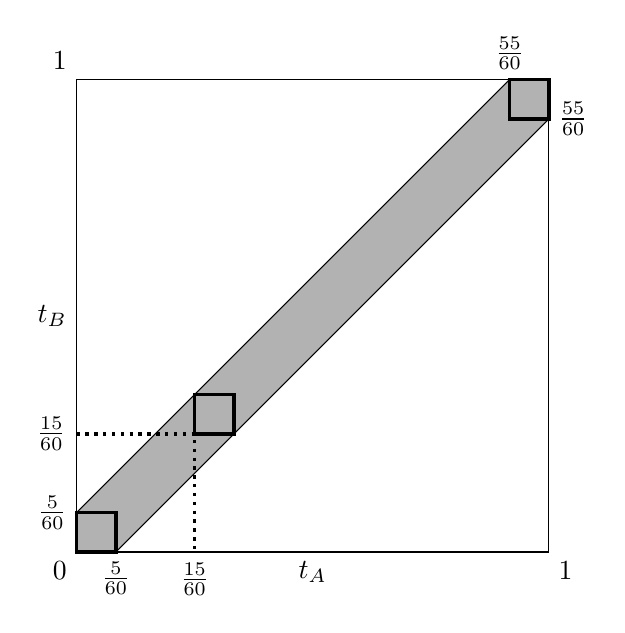
\begin{tikzpicture}
\draw (0,0) -- node[below] {$t_A$} (6,0) -- (6,6) -- (0,6) -- node[left] {$t_B$} cycle;
\node[below left]  at (0,0) {$0$};
\node[below right] at (6,0) {$1$};
\node[above left]  at (0,6) {$1$};
\draw[fill=white!70!black]
  (0,0) -- 
  (.5,0) node[below] {$\frac{5}{60}$} -- 
  (6,5.5) node[right] {$\frac{55}{60}$} --
  (6,6) -- (5.5,6) node[above] {$\frac{55}{60}$} --
  (0,.5) node[left] {$\frac{5}{60}$} -- cycle;
\draw[very thick] (0,0) -- (.5,0) -- (.5,.5) -- (0,.5) -- cycle;
\draw[very thick] (1.5,1.5) -- ++(.5,0) -- ++(0,.5) --
  ++(-.5,0) -- cycle;
\draw[very thick] (5.5,5.5) -- ++(.5,0) -- ++(0,.5) --
  ++(-.5,0) -- cycle;
\draw[very thick,dotted] (0,1.5) node[left] {$\frac{15}{60}$} --
  (1.5,1.5) -- (1.5,0) node[below] {$\frac{15}{60}$};
\end{tikzpicture}
\end{center}
\caption{זמנים המבטיחים מפגש בין $A$ ל-$B$}\label{f.duel}
\end{figure}
אם 
$A$
מגיע יותר מאוחר אזי גם
$B$
חייב להגיע באותו איחור; 
למשל, אם 
$A$
מגיע ב-%
$t_A=15$,
$B$
חייב להגיע בין
$t_B=15$
ו-%
$t_B=20$.
לכן הפגישה תתקיים בריבוע המתקבל על ידי הזזת הריבוע ב-%
$15$
מ-%
$(0,0)$
ל-%
$(15/60,15/60)$.

ההסתברות לפגישה היא היחס בין השטח האפור בגרף לשטח הריבוע הגדול. קל יותר לחשב את המשלים שהוא היחס בין שטח המשולשים הלבנים לשטח הריבוע הגדול:
\begin{eqn}
P(\textrm{נפגשים}\;A,B) &=& 1- P(\textrm{נפגשים לא}\;A,B)\\
&=&1- 2\cdot \left(\frac{1}{2}\cdot \frac{55}{60}\cdot \frac{55}{60}\right)=\frac{23}{144}\approx 0.1597\,.
\end{eqn}

\textbf{סימולציה}
\selectlanguage{english}
\begin{verbatim}
Probability of meeting   = 0.1597
Proportion of meetings   = 0.1549
\end{verbatim}
\selectlanguage{hebrew}

%%%%%%%%%%%%%%%%%%%%%%%%%%%%%%%%%%%%%%%%%%%%%%%%%%%%%%%%%%%%%

\begin{prob}{לתפוס את הזייפן הזהיר}{S}{(Catching the cautious counterfeiter)}

נתון 
$n$
קופסאות ובכל אחת 
$n$
מטבעות כאשר מטבע אחד בכל קופסה מזויף. שלוף מטבע אחד מכל קופסה ובדוק אם הוא מזויף או אמיתי. מה ההסתברות שכל המטבעות שנשלפות מזויפים?

\que{1} 
פתור עבור
$n=10$.

\que{2} 
פתור עבור 
$n=100$.

\que{3}
פתור עבור 
$n$
שרירותי.

\que{4}
פתח נוסחה עבור ההסתברות כאשר
$n$
שואב לאיסוף.
\end{prob}

\solution{}

השליפות בלתי תלויות ולכן ההסתברות היא מכפלת ההסתברות של כל שליפה.

\ans{1}
\[
P(\textrm{אמיתיים המטבעות כל}) = \left(\frac{9}{10}\right)^{10}=0.3487\,.
\]


\ans{2}
\[
P(\textrm{אמיתיים המטבעות כל}) = \left(\frac{99}{100}\right)^{100}=0.3660\,.
\]

\ans{3}
\[
P(\textrm{אמיתיים המטבעות כל}) = \left(\frac{n-1}{n}\right)^{n}\,.
\]

\ans{4}
\begin{equation}\label{eq.reciprocal}
\lim_{n\rightarrow\infty}\left(1-\frac{1}{n}\right)^{n}=\frac{1}{e}\,.
\end{equation}

ניתן להוכיח את הגבול בעזרת חשבון דיפרנציאלי. תחילה ניתן לחשב את הגבול של הלוגריתם של הצד השמולי של משוואה%
~\ref{eq.reciprocal}:
\[
\lim_{n\rightarrow\infty}\ln \left(1-\frac{1}{n}\right)^{n}=
  \lim_{n\rightarrow\infty}n\ln \left(1-\frac{1}{n}\right)=
  \lim_{n\rightarrow\infty} \disfrac{\ln\left(1-\frac{1}{n}\right)}{1/n}\,.
\]
אם נחשב את הגבול נקבל
$(ln \;1)/0=0/0$
אבל לפי חוק
\L{l'H\^{o}pital}
נוכל להחליף את הביטוי בחילוק הנגזרות:
\begin{eqn}
\lim_{n\rightarrow\infty}\ln \left(1-\frac{1}{n}\right)^{n}&=&\lim_{n\rightarrow\infty}\frac{\left(1-\frac{1}{n}\right)^{-1}(-(-n^{-2}))}{-n^{-2}}=-1\\
\lim_{n\rightarrow\infty}\left(1-\frac{1}{n}\right)^{n}&=&e^{-1}\approx 0.3679\,.
\end{eqn}

\textbf{סימולציה}
\selectlanguage{english}
\begin{verbatim}
For  10 boxes:
Probability of all real = 0.3487
Proportion all real     = 0.3480
For 100 boxes:
Probability of all real = 0.3660
Proportion all real     = 0.3730
For 200 boxes:
Probability of all real = 0.3670
Proportion all real     = 0.3690
\end{verbatim}
\selectlanguage{hebrew}

%%%%%%%%%%%%%%%%%%%%%%%%%%%%%%%%%%%%%%%%%%%%%%%%%%%%%%%%%%%%%

\begin{prob}{לתפוס את הזייפן החמדן}{S}{(Catching the greedy counterfeiter)}

נתון 
$n$
קופסאות ובכל אחת 
$n$
מטבעות מהם
$m$
מזוייפים. שלוף מטבע אחת מכל קופסה ובדוק אם הוא מזויף או אמיתי. מה ההסתברות 
$P(n,m,r)$
ש-%
$r$
מתוך המטבעות הם מזוייפים?

\que{1} 
פתח נוסחה עבור
$P(n,m,r)$.

\que{2}
חשב
$P(20,10,2), P(20,10,8), P(20,5,2), P(20,5,4)$.
\end{prob}

\solution{}

\ans{1}
יש 
${n\choose r}$
אוספים של קופסאות מהן המטבעות המזוייפים נשלפו. מההתפלגות הבינומית:
\[
P(n,m,r) = {n \choose r} \left(\frac{m}{n}\right)^r \left(\frac{n-m}{n}\right)^{n-r}\,.
\]

\ans{2}
\begin{eqn}
P(20,10,2) &=& \dischoose{20}{2} \left(\frac{10}{20}\right)^2 \left(\frac{10}{20}\right)^{18}\approx 0.0002\\
P(20,10,8) &=& \dischoose{20}{8} \left(\frac{10}{20}\right)^{8} \left(\frac{10}{20}\right)^{12}\approx 0.1201\\
P(20,5,2)&=&\dischoose{20}{2} \left(\frac{5}{20}\right)^2 \left(\frac{15}{20}\right)^{18}\approx 0.0669\\
P(20,5,4)&=&\dischoose{20}{4} \left(\frac{5}{20}\right)^{4} \left(\frac{15}{20}\right)^{12}\approx 0.1952\,.
\end{eqn}

\L{Mosteller}
מראה שעבור
$m,r$
נתונים, כאשר
$n$
שואף לאינסוף: 
\begin{equation}\label{eq.bin-limit}
\lim_{n\rightarrow \infty}P(n,m,r) = \frac{e^{-m}m^r}{r!}\,.
\end{equation}

\textbf{סימולציה}
\selectlanguage{english}
\begin{verbatim}
For 10 bad coins,  2 draws:
Probability of counterfeit  = 0.0002
Proportion counterfeit      = 0.0002
For 10 bad coins,  8 draws:
Probability of counterfeit  = 0.1201
Proportion counterfeit      = 0.1181
For  5 bad coins,  2 draws:
Probability of counterfeit  = 0.0669
Proportion counterfeit      = 0.0688
For  5 bad coins,  4 draws:
Probability of counterfeit  = 0.1897
Proportion counterfeit      = 0.1905
\end{verbatim}
\selectlanguage{hebrew}

%%%%%%%%%%%%%%%%%%%%%%%%%%%%%%%%%%%%%%%%%%%%%%%%%%%%%%%%%%%%%

\begin{prob}{\protect עובש בג'לטין}{S}{(Moldy gelatin)}

נתון לוח מלבני שמחולק ל-%
$n$
משבצות ריבועיות קטנות. בכל משבצת יש 
$r$ 
חיידקים בממוצע.

\que{1} 
פתח נוסחה להסתברות שיש בדיוק 
$r$
חיידקים ב-%
$n$
המשבצות.

\que{2}
חשב את ההסתברות עבור
$n=100,r=3$.

\textbf{רמז:}
בעיה זו דומה לבעיה~28.

\end{prob}

\solution{}

\ans{1}
תהי 
$p$
ההסתברות שבמשבצת אחת נמצא חידק. (ניתן להתעלם מהאפשרות חידק את מוכל באופן חלקי בשתי משבצות או יותר.) 
$m$,
המספר הממוצע של חיידקים במשבצת, היא מספר המשבצות
$n$
כפול ההסברות 
$p$
שחידק נמצא במשבצת. 
$P(n,m,r)$,
ההסתברות שיש בדיוק 
$r$
חיידקים ב-%
$n$
משבצות ניתנת על ידי ההתפלגות הבינומית:
\[
P(n,m,r) = {n \choose r} \left(\frac{m}{n}\right)^r \left(\frac{n-m}{n}\right)^{n-r}\,.
\]

\ans{2} 
\[
P(10,3,3) = {100 \choose 3} \left(\frac{3}{100}\right)^3 \left(\frac{97}{100}\right)^{97}\approx 0.2275\,.
\]
משוואה%
~\ref{eq.bin-limit}
מתאים גם כאן ולכן:
\[
\lim_{n\rightarrow \infty} P(n,3,3) = \frac{e^{-3}\cdot 3^3}{3!}\approx 0.2240\,.
\]
\textbf{סימולציה}
\selectlanguage{english}
\begin{verbatim}
For  20 squares:
Probability of exactly  3 microbes  = 0.2428
Proportion of exactly   3 microbes  = 0.2436
Probability of exactly  5 microbes  = 0.2023
Proportion of exactly   5 microbes  = 0.1954
For 100 squares:
Probability of exactly  3 microbes  = 0.2275
Proportion of exactly   3 microbes  = 0.2247
Probability of exactly  5 microbes  = 0.1800
Proportion of exactly   5 microbes  = 0.1851
\end{verbatim}
\selectlanguage{hebrew}

%%%%%%%%%%%%%%%%%%%%%%%%%%%%%%%%%%%%%%%%%%%%%%%%%%%%%%%%%%%%%

\refstepcounter{problem} % 30. Evening the sales

%%%%%%%%%%%%%%%%%%%%%%%%%%%%%%%%%%%%%%%%%%%%%%%%%%%%%%%%%%%%%
